\documentclass[../main.tex]{subfiles}

\begin{document}
\section{Parte software}

A parte do software deve permitir o usuário realizar as funções descritas na parte geral.

\subsection{Sistema}
Talvez fazer com que o software seja um sistema operacional direto, evitando acessar o sistema e carregar o aplicativo toda vez que ligar o dispositivo. \newline

\subsection{Funções gerais}
Em geral, cada função listada aqui será um botão na tela principal. \newline

\subsubsection{Pokédex}
Para essa função, permitir ao usuário ver todos os pokémons que está no banco de dados do sistema. Caso o usuário decida ver um pokémon em específico, demonstrar informações, sprite e permitir adicionar na equipe do usúario.\newline

\begin{figure}[H]
\centering
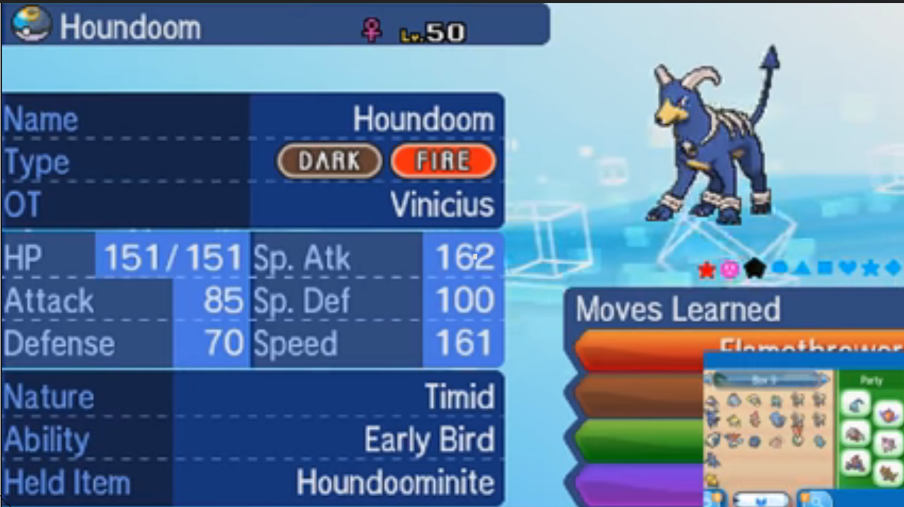
\includegraphics[scale=0.5]{../Images/softwarePokedexInfo.png}
\caption{Visualização de informação referente a um pokémon em especifico.}
\end{figure}


\subsubsection{Pokémon}
Para essa função, permitir ao usuário ver a sua equipe pokémon, com informações e outros. \newline

\begin{figure}[H]
\centering
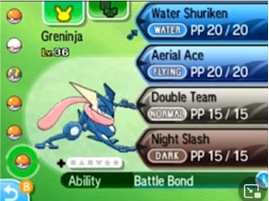
\includegraphics[scale=1]{../Images/softwareTeam.png}
\caption{Visualização da equipe pokémon.}
\end{figure}

\subsubsection{Bag}
Para essa função, permitir ao usuário ver os items que podem aparecer no jogo. \newline

Como a maioria dos items aparecem depois de coletado e/ou comprados, seria ideal apenas mostrar o item e informações relacionados. \newline

\begin{figure}[H]
\centering
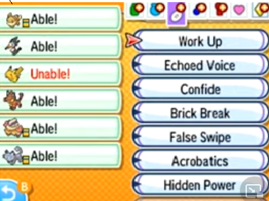
\includegraphics[scale=1]{../Images/softwareBag.png}
\caption{Visualização de bag.}
\end{figure}

\subsubsection{Save}
Permitir que o usuário "Salve" o jogo, o qual irá registrar a equipe decidida e fazer a animação de salvando o jogo. \newline

\subsubsection{Câmera}
Permitir ao usuário usar a câmera do dispositivo. \newline

\subsubsection{Fotos}
Permitir ao usuário ver as fotos tiradas. \newline

\subsection{Sugestões}
- Incluir um clock \newline
- Permitir ao usuário ver o quanto de bateria ainda tem disponível \newline
- Permitir ao usuário enviar as fotos do dispositivo para o PC. \newline

\subsection{Recursos}

\subsubsection{Imagens, pokemon e outros}
\url{https://pokeapi.co/}

\subsubsection{Imagens usadas para esse capítulo}
\href{https://www.youtube.com/watch?v=g2Jbhj6MhMk}{Vídeo}

\subsubsection{Links em gerais}
\href{https://www.linuxfromscratch.org/}{Linux from scratch}
\href{https://worproject.ml/}{Windows for raspberry}



\end{document}